\documentclass[a4paper,oneside,openright]{memoir}

\usepackage{dangkhoa}

\title{Độ tương tự hành vi của chương trình \\và thực nghiệm}
\author{Đỗ Đăng Khoa}

\begin{document}

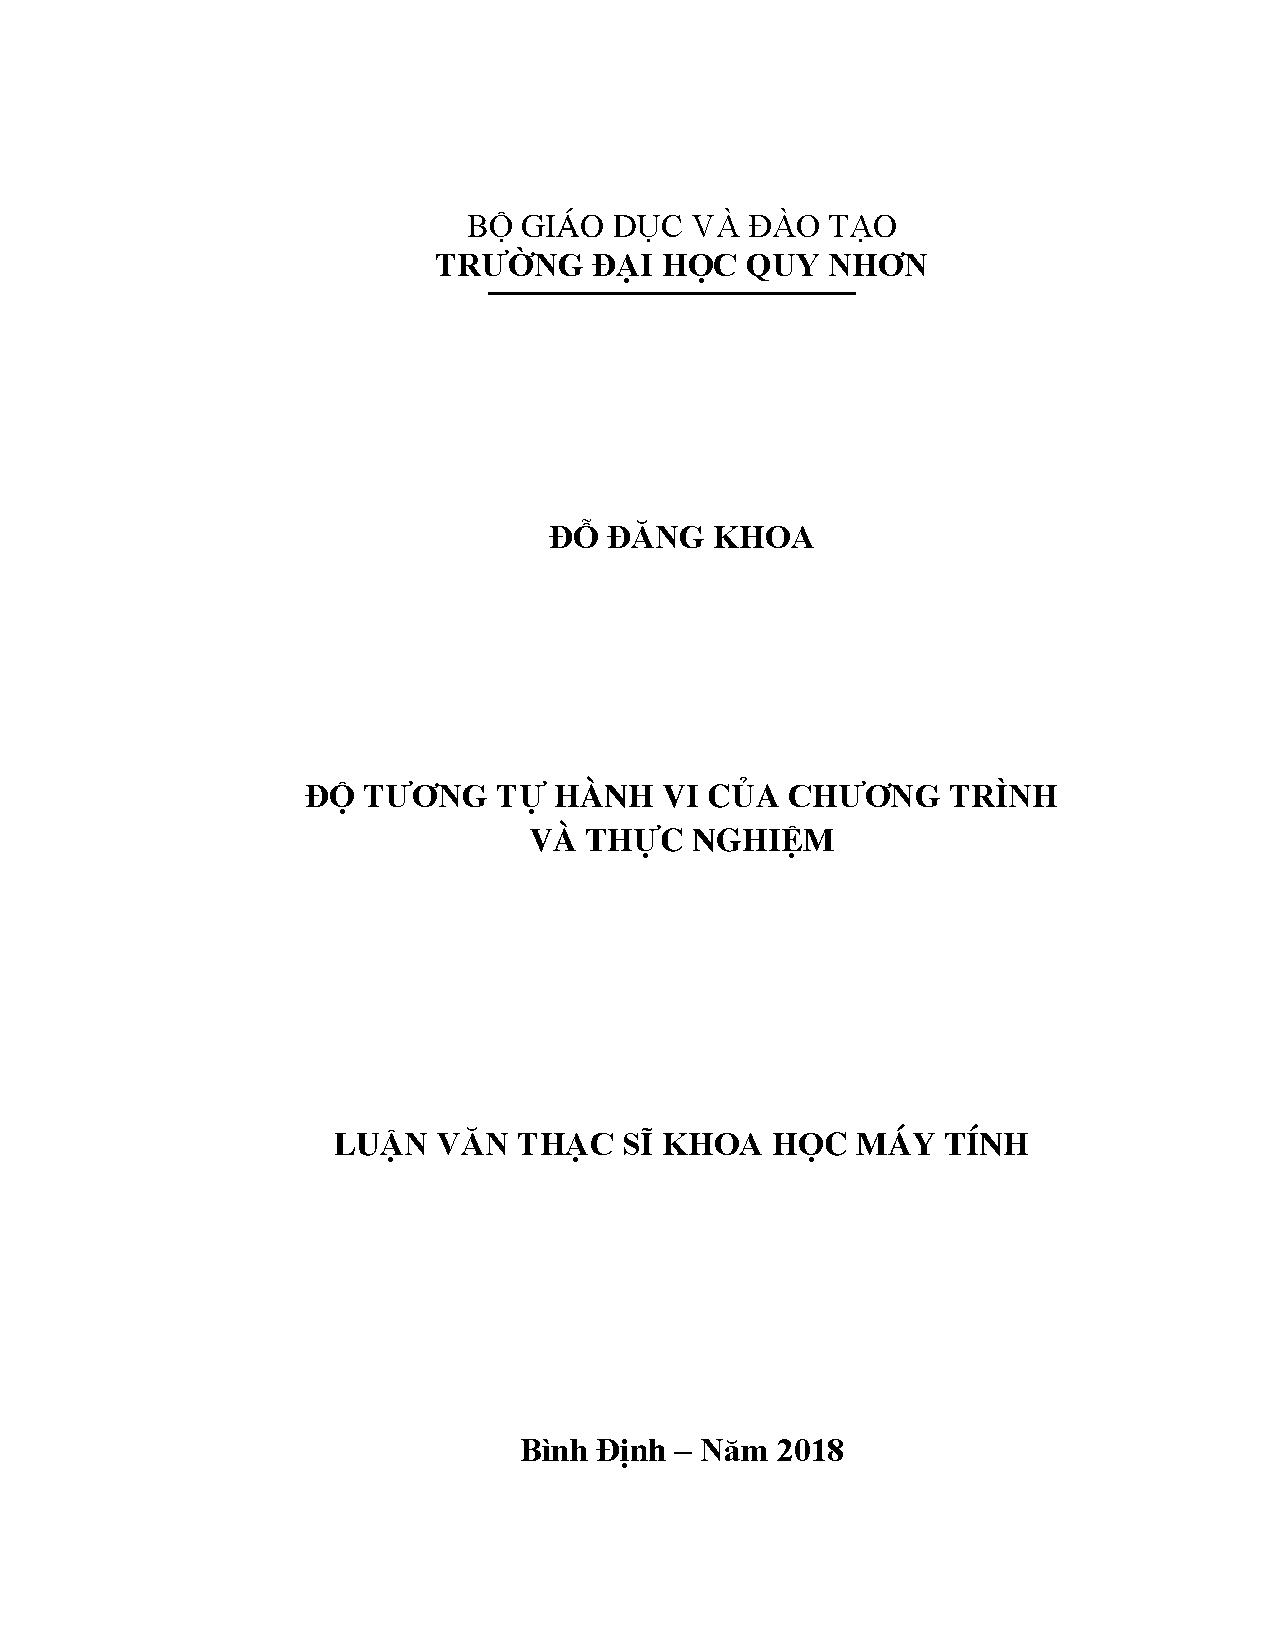
\includepdf[pages=-]{trangbia.pdf}

% \pagenumbering{gobble} % Trước trang không đánh số thứ tự 

% \pagenumbering{roman} % Trước trang đánh số la mã
% \setcounter{page}{1}

\chapter*{Lời cam đoan}
\input{Loicamdoan}

\chapter*{Lời cảm ơn}

Tôi xin chân thành cảm ơn sự hướng dẫn, chỉ dạy và giúp đỡ tận tình của các thầy cô giảng dạy sau đại học - Trường đại học Quy Nhơn.

Đặc biệt, tôi cảm ơn thầy TS.Phạm Văn Việt, giảng viên bộ môn Công nghệ phần mềm, khoa Công nghệ thông tin, Trường Đại học Quy Nhơn đã tận tình hướng dẫn truyền đạt những kiến thức và kinh nghiệm quý báu đễ giúp tôi có đầy đủ kiến thức và nghị lực hoàn thành luận văn này.

Và tôi xin cảm ơn bạn bè, đồng nghiệp và những người thân trong gia đình đã tin yêu, động viên giúp tôi thêm nghị lực trong quá trình học tập và nghiên cứu.

Mặc dù đã cố gắng rất nhiều trong việc thực hiện luận văn, song với thời gian có hạn, nên luận văn không thể tránh khỏi những thiếu sót và chưa hoàn chỉnh. Tôi rất mong nhận được ý kiến đóng góp của quý Thầy Cô và các bạn.

Một lần nữa, tôi xin chân thành cảm ơn!.


\begin{tabu} to 1.0 \textwidth {  X[c] X[c]  X[c]  X[c]  }

	 & &  & \textbf{HỌC VIÊN} \\
	 \\ \\ \\ \\ \\ \\ \\ \\ \\ \\ \\ 
	 & &  & \textbf{Đỗ Đăng Khoa}  \\
         
       \end{tabu}




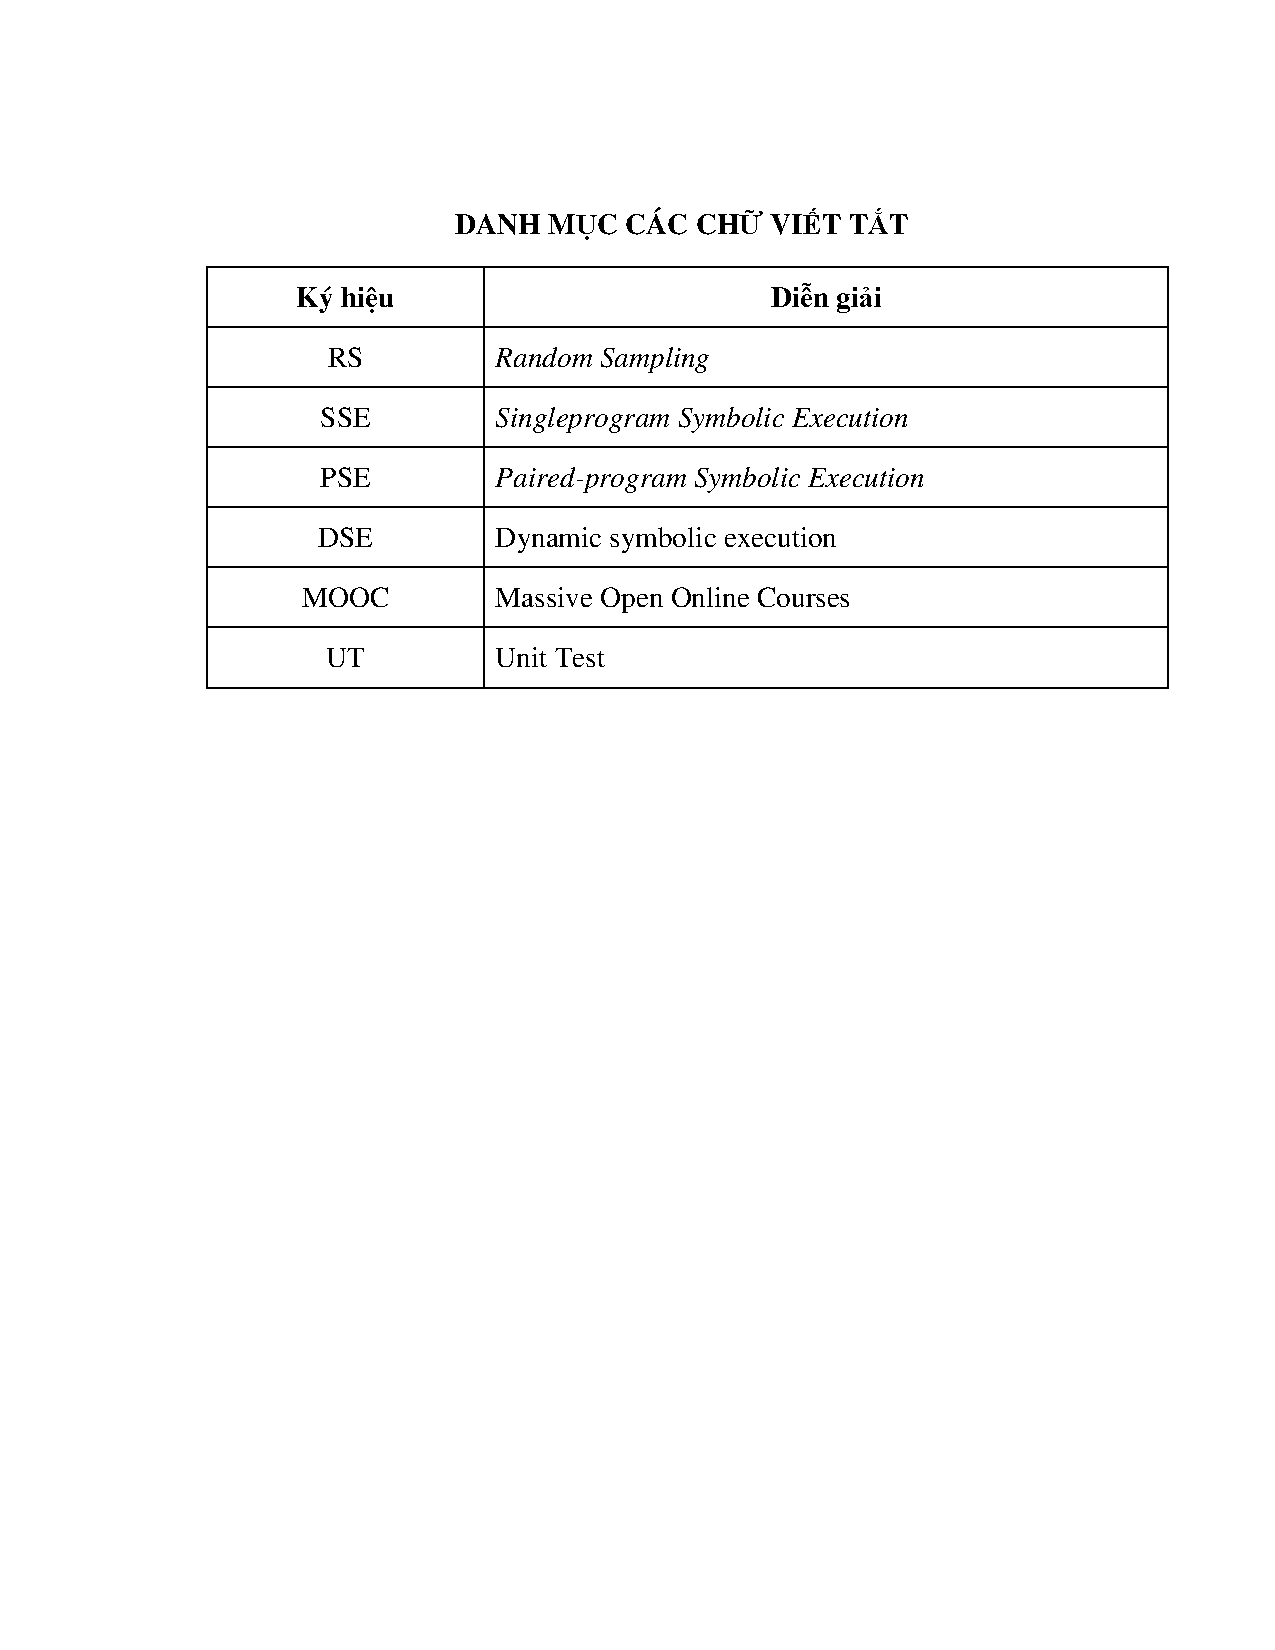
\includepdf[pages=-]{Danhmuckyhieu.pdf}

\newpage
\tableofcontents

%======================================================================
% \pagenumbering{arabic} % Trước trang đánh số thứ tự thêm 2 dòng này
% \setcounter{page}{1}   % Trước trang đánh số thứ tự thêm 2 dòng này - số trang bắt đầu bằng 3


\includepdf[pages=-]{Tomtat.pdf}

\chapter{Giới thiệu}
\newpage
\chapter{GIỚI THIỆU}

\section{Lý do chọn đề tài, ngữ cảnh bài toán}
		
Trong những năm gần đây, xu hướng đào tạo lập trình viên nói riêng và công nghệ phần mềm nói chung đang ngày càng trở nên phổ biến. Các trường đại học và một số trung tâm đào tạo đã cho ra đời nhiều chương trình đào tạo phong phú về nội dung, đa dạng về hình thức và thu hút được nhiều sự quan tâm.\\
	
Trong mỗi khóa học, số lượng học viên thường có hằng trăm, hằng ngàn người tham gia, nhưng chỉ một vài giáo viên giảng dạy. Trong đó, chất lượng việc quản lý, truyền đạt nội dung của giáo viên và mức độ hiểu biết, nắm bắt nội dung chương trình học của học viên là yêu cầu tất cả các khóa học cần đạt được. Để đạt được điều đó, một yêu cầu bắt buộc đó là giáo viên phải đọc và hiểu tất cả các đoạn code của học sinh, nhưng công việc này lại tốn quá nhiều thời gian. Nếu bỏ qua hoặc trì hoãn các công việc như vậy thì người dạy không thể theo dõi được quá trình học tập của người học. Về phía người học, yêu cầu đặt ra là phải tiến bộ theo thời gian, nắm vững lý thuyết và thành thạo kỹ năng lập trình. Những không phải lúc nào gặp khó khăn người học đều có sự hỗ trợ kịp thời từ giảng viên. Họ có thể nhờ sự giúp đỡ từ đồng nghiệp, bạn bè, nhưng những người được nhờ hiups đỡ chưa chắc đã đủ trình độ, kinh nghiệm hoặc thời gian để ngồi bên cạnh giúp đỡ người học khi cần.\\
	
Để giảm bớt những khó khăn nêu trên, một công cụ hỗ trợ quá trình giảng dạy và học tập của giáo viên và học sinh hiệu quả hơn, tiết kiệm thời gian hơn đó là một công cụ tự động hóa (có thể một phần) việc đánh giá kết quả lập trình của học sinh, cũng như hỗ trợ theo giõi sự tiến bộ của học sinh. Công cụ tự động hóa này sẽ tính toán, định lượng tỷ lệ chính xác sự tương tự về hành vi giữa chương trình của người học và chương trình của người dạy đưa ra trước đó. Dựa trên kết quả, giáo viên sẽ đánh giá được kỹ năng lập trình của học sinh, sự giống nhau giữa hai chương trình càng cao thì tỷ lệ độ tương tự càng cao, điểm số càng cao. Nếu điểm số thấp, người học có thể quay lại kiểm tra để viết mã chương trình đúng hơn, hạn chế được nguy cơ tìm ẩn trong cách viết chương trình của người học.\\
	
Những đánh giá này có thể thực hiện được nếu ta đo được độ tương tự giữa các chương trình có độ chính xác cao. Đề tài “Độ tương tự về hành vi của các chương trình và làm thực nghiệm”  với mục đích sẽ giải quyết các vấn đề nếu trên.

\section{Những nghiên cứu có liên quan}

\chapter{Kiến thức cơ sở}
Chương này trình bày những kiến thức cơ sở để triển khai luận văn này, gồm:
\begin{itemize}
\item Kiểm thử phần mềm,
\item Sinh ngẫu nhiên dữ liệu thử,
\item Kỹ thuật Dynamic Symbolic Execution.
\end{itemize}

\section{Kiểm thử phần mềm}

\cite{myers2011art,whittaker2000software,ammann2016introduction}

\subsection{Giới thiệu}
Trong nền kinh tế hiện nay, ngành công nghiệp phần mềm giữ vai trò hết sức quan trọng. Với một số nước có nền công nghệ thông tin phát triển thì ngành công nghiệp phần mềm có khả năng chi phối cả nền kinh tế. Tuy nhiên để đảm bảo chất lượng cho các phần mềm là một thách thức không nhỏ trong ngành công nghiệp phần mềm. Việc phát hiện và khắc phục các lỗi cho các phần mềm là một công việc đòi hỏi nhiều nỗ lực và chi phí trong phát triển phần mềm. Với những lĩnh vực ứng dụng ngày càng mở rộng của phần mềm hiện nay thì  một sản phẩm phần mềm có thể được nhiều người sử dụng biết đến, nó mang lại hiệu quả tích cực trong công việc của người sử dụng. Tuy nhiên, một phần mềm lỗi sẽ ảnh hưởng đến người sử dụng, gây thiệt hại về kinh tế cũng như ảnh hưởng đến tiến độ công việc của người sử dụng. Phần mềm phải luôn đảm bảo được sự ổn định, không phát sinh lỗi, tránh gây ảnh hưởng tới người sử dụng.

Việc kiểm thử phần mềm chính là một quá trình hoặc một loạt các quy trình được thiết kế, để đảm bảo mã máy tính chỉ làm những gì nó được thiết kế và nó không làm bất cứ điều gì ngoài ý muốn \cite{myers2011art}. Phần mềm phải được dự đoán, nhất quán và không gây bất ngờ cho người dùng. Đây là một bước quan trọng trong quá trình phát triển một phần mềm, giúp cho người phát triển phần mềm và người sử dụng thấy được hệ thống đã đáp ứng yêu cầu đặt ra.

\subsection{Các phương pháp kiểm thử}
\textbf{\textit{Kiểm thử tĩnh (Static testing)}}: Là phương pháp kiểm thử phần mềm bằng cách duyệt lại các yêu cầu và các đặc tả bằng tay, thông qua việc sử dụng giấy, bút để kiểm tra tính logic từng chi tiết mà không cần chạy chương trình. Kiểu kiểm thử này thường được sử dụng bởi chuyên viên thiết kế, người viết mã lệnh chương trình. Kiểm thử tĩnh cũng có thể được tự động hóa bằng cách thực hiện kiểm tra toàn bộ hệ thống thông qua một trình thông dịch hoặc trình biên dịch, xác nhận tính hợp lệ về cú pháp của chương trình.
		
\textbf{\textit{Kiểm thử động (Dynamic testing)}}: Là phương pháp kiểm thử thông qua việc chạy chương trình để điều tra trạng thái tác động của chương trình, dựa trên các ca kiểm thử xác định các đối tượng kiểm thử của chương trình. Đồng thời kiểm thử động sẽ tiến hành kiểm tra cách thức hoạt động của mã lệnh, tức là kiểm tra phản ứng từ hệ thống với các biến luôn thay đổi theo thời gian. Trong kiểm thử động, phần mềm phải được biên dịch và chạy, và bao gồm việc nhập các giá trị đầu vào và kiểm tra giá trị đầu ra có như mong muốn hay không.	
	
\subsection{Các chiến lược kiểm thử}

Trong chiến lược kiểm thử, đề tài quan tâm đến hai chiến lược kiểm thử đó là kiểm thử hộp đen, kiểm thử hộp trắng.
	
\textbf{\textit{Kiểm thử hộp đen – Black box}}. Đây là một trong những cách kiểm thử quan trọng, cách thức hoạt động chủ yếu dựa vào hướng dữ liệu inputs/ouputs của chương trình, xem chương trình như là một “hộp đen” và hoàn toàn không quan tâm về cách xử lý, cũng như cấu trúc bên trong của chương trình. Kiểm thử hộp đen tập trung vào tìm các trường hợp mà chương trình không thực hiện theo các đặc tả kỹ thuật. Kiểm thử viên hộp đen sẽ cố gắng tìm ra những lỗi mà những lập trình viên không tìm ra. Nhưng phương pháp kiểm thử này cũng có mặt hạn chế của nó, kiểm thử viên không biết các phần mềm được kiểm tra thực sự được xây dựng như thế nào, cố gắng viết rất nhiều ca kiểm thử để kiểm tra một thứ gì đó mà đáng lẽ chỉ cần kiểm tra bằng một ca kiểm thử duy nhất, hoặc một số phần của chương trình có thể bị bỏ qua không được kiểm tra.
		
Do vậy, kiểm thử hộp đen có ưu điểm là đánh giá khách quan, mặt khác nó lại có nhược điểm là thăm dò mù. Trong phần nghiên cứu của đề tài, kiểm thử hộp đen cũng được sử dụng như một phương pháp đo độ tương tự hành vi của các chương trình.
		
\textbf{\textit{Kiểm thử hộp trắng – White box}}. Đây là một chiến lược kiểm thử khác, trái ngược hoàn toàn với kiểm thử hộp đen, kiểm thử hộp trắng hay còn gọi là kiểm thử hướng logic của phần mềm. Cách kiểm thử này cho phép tạo ra dữ liệu thử nghiệm từ việc kiểm tra, khảo sát cấu trúc bên trong và kiểm thử tính logic của chương trình. Dữ liệu thử nghiệm có độ phủ lớn, đảm bảo được tất cả các đường dẫn, hoặc các nhánh của chương trình được thực hiện ít nhất một lần, khắc phục được những nhược điểm thăm dò mù trong cách kiểm thử hộp đen.
		
Phương pháp kiểm thử hộp trắng cũng có thể được sử dụng để đánh giá một bộ kiểm thử được tạo với các phương pháp kiểm thử hộp đen. Trong các phép đo độ tương tự của đề tài, phương pháp kiểm thử hộp trắng là một phương pháp quan trọng, được áp dụng để đo hành vi của các chương trình.
	
\subsection{Các cấp độ kiểm thử trong kiểm thử phần mềm}
Kiểm thử phần mềm gồm có các cấp độ: 
\begin{itemize}
	\item Kiểm thử đơn vị
	\item Kiểm thử tích hợp
	\item Kiểm thử hệ thống
	\item Kiểm thử chấp nhận sản phẩm
\end{itemize}
	
\begin{center}
	\begin{figure}[htp]
		\begin{center}
			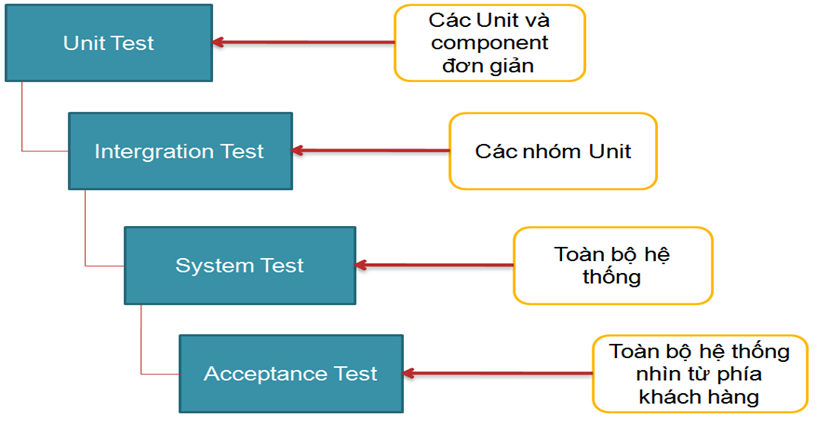
\includegraphics[scale=.3]{giai-doan-kiem-thu-1.png}
		\end{center}
		\caption{Sơ đồ các cấp độ kiểm thử}
		\label{refhinh1}
	\end{figure}
\end{center}
	
\subsection{Đảm bảo chất lượng phần mềm}
\textbf{Định nghĩa theo Daniel Galin \cite{galin2004software}:} Đảm bảo chất lượng phần mềm là một tập hợp các hành động được lên kế hoạch một cách hệ thống để cung cấp đầy đủ niềm tin rằng quá trình phát triển phần mềm phù hợp để thành lập các yêu cầu chức năng kỹ thuật cũng như các yêu cầu quản lý theo lịch trình và hoạt động trong giới hạn.


\section{Sinh ngẫu nhiên dữ liệu thử}
%Phần này trình bày cơ bản về sinh dữ liệu thử ngẫu nhiên, những ưu và nhược điểm cùng những cải tiến để nâng cao hiệu quả.
Sinh ngẫu nhiên dữ liệu thử là một kỹ thuật kiểm thử phần mềm Black-Box kỹ thuật này tạo ra ngẫu nhiên các giá trị đầu vào và thực thi từng giá trị đầu vào này trên chương trình được kiểm thử. Kết quả của đầu ra được so sánh với các thông số kỹ thuật của phần mềm, để xác định đầu ra thử nghiệm thành công hoặc không thành công \cite{myers2011art}.  

Kỹ thuật này không quan tâm đến hành vi và cấu trúc bên trong của chương trình, chỉ tập trung tìm kiếm những trường hợp chương trình không hoạt động theo đặc tả kỹ thuật của chương trình. Trong phương pháp này, dữ liệu thử nghiệm được tạo ngẫu nhiên từ các đặc tả kỹ thuật của phần mềm (tức là không liên quan tới hành vi và cấu trúc của chương trình).

\subsection*{Ví dụ:}
\lstinputlisting[caption = {Hàm sinh ngẫu nhiên dữ liệu thử}]{RandomTesting.cs}
Đây là một hàm sinh ngẫu nhiên dữ liệu thử, chúng ta thấy hàm \textbf{testAbs} chỉ thực hiện việc tạo giá trị đầu vào ngẫu nhiên \textbf{int x} theo đặc tả tham số đầu vào của chương trình \textbf{myAbs}, và kiểm tra kết quả đầu ra của chương trình \textbf{assert(result >= 0)}, không quan tâm hành vi và cấu trúc bên trong của hàm \textbf{myAbs}.

\subsection*{Ưu điểm và hạn chế}

\textit{* Ưu điểm:}
\begin{itemize}
	\item Đơn giản, dễ dàng sinh các đầu vào ngẫu nhiên
	\item Không tốn nhiều tài nguyên bộ nhớ lúc thực thi
\end{itemize}

\textit{* Hạn chế:}
\begin{itemize}
	\item Một nhánh hành vi của chương trình được kiểm thử nhiều lần với nhiều đầu vào khác nhau
	\item Có thể một số nhánh hành vi của chương trình bị bỏ qua
	\item Khó xác định khi nào việc kiểm thử nên dừng lại
	\item Không biết dữ liệu thử có duyệt được tất cả các nhánh trong chương trình hay không
\end{itemize}

\subsection*{Hướng khác phục}
Để xác định khi nào việc kiểm thử dừng lại, hệ thống kiểm thử ngẫu nhiên có thể kết hợp với các kỹ thuật Adequacy Criterion \cite{zhu1997software}. Kỹ thuật Adequacy Criterion là một kỹ thuật yêu cầu duyệt tất cả các nhánh của chương trình, bằng việc kết hợp này cho phép việc kiểm thử chỉ dừng lại khi tất cả các câu lệnh của chương trình được thực thi ít nhất một lần.

Một kỹ thuật khác giúp khắc phục được hạn chế của kiểm thử ngẫu nhiên đó là kỹ thuật thực thi tượng trưng \cite{king1976symbolic}. Thực thi tượng trưng là một kỹ thuật xây dựng các ràng buộc dựa vào các điều kiện tại các nút nhánh của chương trình, giải quyết các ràng buộc đó để sinh ra các giá trị  đầu của chương trình. Thực thi các giá trị đầu vào này, chúng ta có thể duyệt được tất cả các nhánh của chương trình. 


\section{Kỹ thuật Dynamic symbolic execution}
% What? 
% why?
% how?
% who?

Dynamic symbolic execution (DSE) là một kỹ thuật duyệt tự động tất cả các đường đi có thể của chương trình bằng cách chạy chương trình với nhiều giá trị đầu vào khác nhau để tăng độ phủ của dữ liệu thử \cite{xie2009fitness}.

Dựa trên các tham số đầu vào của chương trình, DSE sẽ tạo ra các giá trị đầu vào cụ thể và thực thi chương trình với các giá trị cụ thể này. Trong quá trình thực thi, DSE sẽ ghi nhận lại ràng buộc tại các nút, phủ định lại các ràng buộc này và sinh các giá trị đầu vào thỏa điều kiện ràng buộc tại các nút rẽ nhánh này. Với một giá trị đầu vào cụ thể, DSE sẽ thực thi chương trình và duyệt được một đường đi cụ thể, quá trình thực thi này sẽ lặp lại cho đến khi duyệt hết tất cả các đường đi của chương trình.

\subsection*{Thuật toán}
\begin{center}
	\begin{figure}[htp]
		\begin{center}
			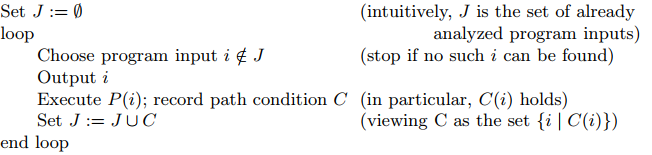
\includegraphics[scale=.7]{thuat_toan_DSE.png}
		\end{center}
		\caption{Thuật toán kỹ thuật DSE}
		\label{refhinh1}
	\end{figure}
\end{center}


\subsection*{Ví dụ:}

\lstinputlisting[caption = {Minh họa kỹ thuật DSE}]{DSE.cs}
	
Trong ví dụ trên, chúng ta xem xét hàm \textbf{test\_me} với hai tham số đầu vào là \textbf{int x} và \textbf{int y}, và hàm này không có giá trị trả về. Cách thức làm việc của DSE trên hàm \textbf{test\_me} như sau: 

Đầu tiên, DSE tạo hai giá trị đầu vào ngẫu nhiên \textbf{x} và \textbf{y}, giả sử \textbf{x = 22} và \textbf{y = 7}. Ngoài ra, DSE sẽ theo dõi trạng thái các giá trị đầu vào của chương trình: \textbf{x} bằng một tham số \textbf{x\_0} và \textbf{y} bằng một tham số \textbf{y\_0}.

Ở dòng đầu tiên, số nguyên \textbf{z} được gán bằng hàm \textbf{foo(y)}. Điều này có nghĩa là \textbf{z} bây giờ bằng 14, và ở trạng thái tượng trưng, biến \textbf{z} có giá trị \textbf{2*y\_0}. 

Tại điểm nhánh \textbf{“z == x”}, DSE nhận biết giá trị của \textbf{x} không bằng giá trị của \textbf{z}. Về mặt biểu tượng, DSE lưu trữ ràng buộc này là \textbf{(z != x)}, và điều kiện đường dẫn sẽ là: \textbf{2*y\_0 != x\_0}. DSE sau đó đi theo nhánh “\textbf{false}” dẫn đến kết thúc chương trình.

Sau khi kết thúc chương trình, DSE sẽ quay trở lại điểm nhánh gần nhất và cố gắng chọn nhánh "true". Với mục đích này, nó phủ định ràng buộc được thêm gần nhất trong điều kiện đường dẫn \textbf{2*y\_0 != x\_0} thành \textbf{2*y\_0 == x\_0}. Để thỏa mãn ràng buộc \textbf{2*y\_0 != x\_0}, hai số nguyên thỏa mãn ràng buộc này được trả về là \textbf{x\_0 = 2 }và\textbf{ y\_0 = 1}.


\begin{center}
	\begin{figure}[htp]
		\begin{center}
			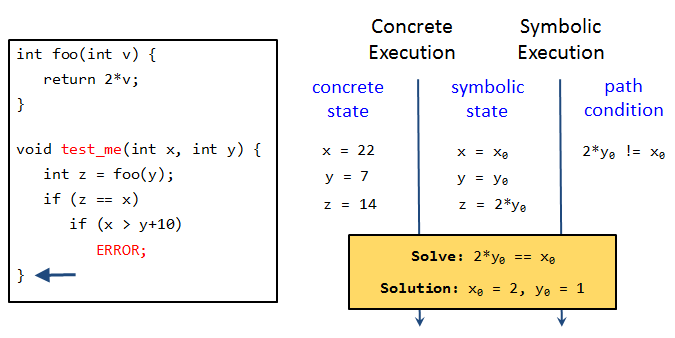
\includegraphics[scale=.4]{dse2.png}
		\end{center}
		\caption{Các giá trị DSE sinh ra sau khi thực thi chương trình lần 1}
		\label{refhinh1}
	\end{figure}
\end{center}

Sau đó, DSE khởi động lại hàm \textbf{test\_me}, lần này nó gọi các giá trị đầu vào cụ thể được tạo ra bởi quá trình giải quyết ràng buộc: \textbf{x = 2} và \textbf{y = 1}. DSE tiếp tục theo dõi trạng thái các biến với \textbf{x = x\_0} và \textbf{y = y\_0}.

Sau khi thực hiện dòng đầu tiên, \textbf{z} có giá trị cụ thể 2 và giá trị biểu tượng 2*y\_0\textbf{}.

Ở dòng kế tiếp, chúng ta kiểm tra tình trạng nhánh \textbf{z == x}. Trong trường hợp này, điều kiện là đúng, vì vậy điều kiện đường dẫn của chúng ta trở thành \textbf{2*y\_0 == x\_0}. Sau đó \textbf{DSE} kiểm tra dòng tiếp theo của nhánh \textbf{"true"}.

Tại điểm nhánh tiếp theo, \textbf{x} có giá trị cụ thể là 2 và \textbf{y + 10} có giá trị cụ thể là 11, vì vậy \textbf{DSE} lấy nhánh \textbf{"false"}, kết thúc chương trình. Thêm ràng buộc tượng trưng \textbf{x\_0 <= y\_0 + 10} vào điều kiện đường dẫn, là sự phủ định của điều kiện nhánh mà \textbf{DSE} phát hiện là \textbf{fasle}.

Vì DSE đã đến cuối chương trình, nó phủ nhận ràng buộc được thêm gần nhất trong điều kiện đường dẫn để có được \textbf{x\_0> y\_0 + 10}, và sau đó nó vượt qua các ràng buộc \textbf{2*y\_0 == x AND x\_0> y\_0 + 10}. Để thỏa những ràng buộc này, \textbf{DSE} trả về \textbf{x\_0 = 30} và \textbf{y\_0 = 15}.

\begin{center}
	\begin{figure}[htp]
		\begin{center}
			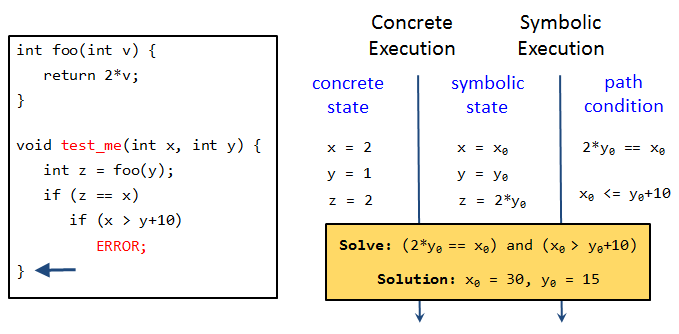
\includegraphics[scale=.4]{dse3.png}
		\end{center}
		\caption{Các giá trị DSE sinh ra sau khi thực thi chương trình lần 2}
		\label{refhinh1}
	\end{figure}
\end{center}

Bây giờ, DSE chạy hàm \textbf{test\_me} một lần nữa, lần này với các đầu vào \textbf{x = 30} và \textbf{y = 15}. Trạng thái biểu tượng các biến bắt đầu \textbf{x = x\_0} và \textbf{y = y\_0}. \textbf{z} được gán giá trị cụ thể 30, trong khi giá trị ký hiệu của nó là \textbf{2*y\_0}, như trước những lần chạy trước.

Khi tới điều kiện rẻ nhánh \textbf{"z == x"}, DSE nhận thấy đây là điều kiện \textbf{true}, vì vậy DSE thêm điều kiện tượng trưng \textbf{2*y\_0 == x\_0}.

Sau đó, tại điểm nhánh tiếp theo, giá trị cụ thể của \textbf{x > y + 10}, vì vậy DSE thêm ràng buộc tượng trưng mới \textbf{x\_0 > y\_0 + 10}. Nhánh này dẫn đến \textbf{"ERROR"}, tại thời điểm đó chúng ta đã xác định được đầu vào cụ thể làm cho chương trình\textbf{"ERROR"} là: \textbf{x = 30} và \textbf{y = 15}.

\begin{center}
	\begin{figure}[htp]
		\begin{center}
			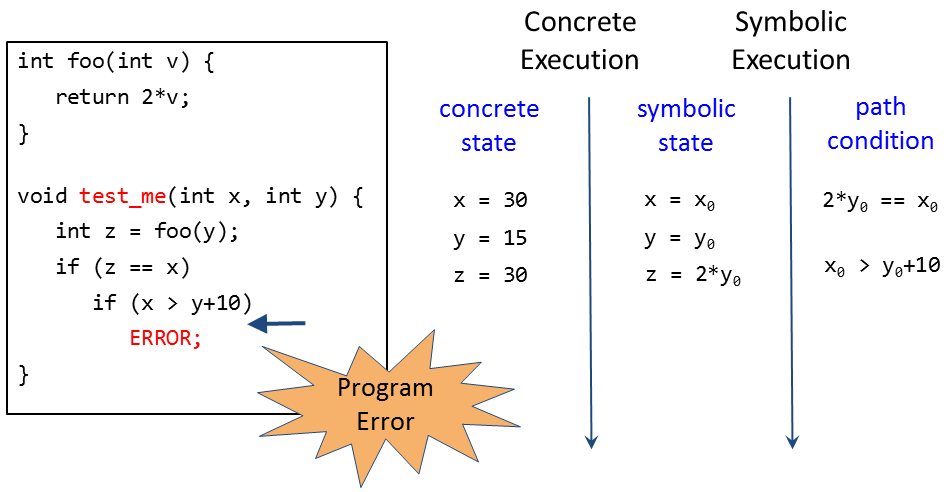
\includegraphics[scale=.4]{dse4.png}
		\end{center}
		\caption{Các giá trị DSE sinh ra sau khi thực thi chương trình lần 3}
		\label{refhinh1}
	\end{figure}
\end{center}

Kết quả, sau 3 lần chạy chương trình, DSE tạo ra được các cặp giá trị đầu vào có thể duyệt hết các nhánh của chương trình \textbf{test\_me} đó là: \textbf{[22,7], [2,1], [30,15]}
	
\subsection{Một số công cụ ứng dụng DSE}	
Hiện nay, trên thế giới có nhiều công cụ sử dụng kỹ thuật DSE để giải quyết các ràng buộc và tạo ra các giá trị đầu vào có độ phủ cao như như Pex \cite{tillmann2008pex} và SAGE \cite{godefroid2008automated}... và một công cụ có thể sử dụng được trên nhiều ngôn ngữ, nền tảng khác nhau.
		
	\begin{center}
		\begin{tabular}  {|c|c|c|} 
			\hline 
			\textbf{Tên Công cụ} & \textbf{Ngôn ngữ} & \textbf{Url} \\ 
			\hline 
			KLEE & LLVM & klee.github.io/ \\ 
			\hline 
			JPF	 & Java	& babelfish.arc.nasa.gov/trac/jpf \\
			\hline 
			jCUTE &	Java &	github.com/osl/jcute \\
			\hline 
			janala2	 & Java &	github.com/ksen007/janala2 \\
			\hline 
			JBSE	& Java	 & github.com/pietrobraione/jbse \\
			\hline 
			KeY &	Java &	www.key-project.org/ \\	
			\hline 
			Mayhem & 	Binary &	forallsecure.com/mayhem.html \\
			\hline 
			Otter &	C	& bitbucket.org/khooyp/otter/overview \\
			\hline 
			Rubyx & 	Ruby &	www.cs.umd.edu/~avik/papers/ssarorwa.pdf \\
			\hline 
			Pex	& .NET Framework	 & research.microsoft.com/en-us/projects/pex/ \\
			\hline 
			Jalangi2 &	JavaScript &	github.com/Samsung/jalangi2 \\
			\hline 
			Kite &	LLVM &	www.cs.ubc.ca/labs/isd/Projects/Kite/ \\
			\hline 
			pysymemu &	x86-64 / Native	 &github.com/feliam/pysymemu/ \\
			\hline 
			Triton	& x86 and x86-64 &	triton.quarkslab.com \\	
			\hline 
			BE-PUM &	x86	 & https://github.com/NMHai/BE-PUM	 \\	
			\hline
			
		\end{tabular} 

	\end{center}
	
\section*{Tổng kết chương}
%Tổng kết chương viết ở đây.
Chương này, trình bày khái quát và sơ lượt những kiến thức như: Kỹ thuật kiểm thử phần mềm; các kỹ thuật sinh dữ liệu thử; kỹ thuật Dynamic symbolic execution. Những kiến thức này, giúp chúng ta có cái nhìn tổng quan về cách thức kiểm thử phần mềm, giải quyết các ràng buộc trong chường trình nhằm tăng độ phủ cho các giá trị đầu vào thử nghiệm.




\chapter{Đo độ tương tự về hành vi giữa các chương trình}
Chương này trình bày một số định nghĩa và các phép đo đo được sử dụng trong luận văn bao gồm:
\begin{itemize}	
	\item Định nghĩa thực thi chương trình
	\item Định nghĩa tương đương hành vi
	\item Định nghĩa sự khác biệt về hành vi
	\item Định nghĩa độ tương tự hành vi
	\item Phép đo Random Sampling (RS)
	\item Phép đo Single Program Symbol Execution (SSE)
	\item Phép đo Paired Program Symbolic Execution
	\item Tiêu chí đánh giá các phép đo.
\end{itemize}

\section{Hành vi của chương trình}
Để định lượng hai chương trình tương tự nhau, chúng ta định nghĩa các khái niệm về hành vi chương trình và các định nghĩa liên quan đến sự tương tự của hai chương trình, và ví dụ minh họa cho các định nghĩa. 
	
\subsection{Thực thi chương trình}
\begin{definition}\label{def:progexe}
Hành vi chương trình P là thực hiện hàm: P $\times$ I $\rightarrow$ O. Với giá trị đầu vào i $\in$ I, giá trị đầu ra o $\in$ O. Trong đó I là miền các trị đầu vào của chương trình P và O là tập hợp các giá trị đầu ra của chương trình P.  
\end{definition}

\subsection{Tương đương hành vi}
\begin{definition}
  Hai chương trình $P_{1}$ và $P_{2}$ có cùng một miền các giá trị đầu
  vào I và tương đương về hành vi nếu exec($P_{1}$; I) = exec($P_{2}$;
  I), với $\forall$i $\in$ I exec($P_{1}$; i) = exec($P_{2}$; i).
\end{definition}
	
\subsubsection{Ví dụ:}

\lstinputlisting[caption = {Tính y, sử dụng hàm Switch...Case}]{SwitchCase.cs}

\lstinputlisting[caption = {Tính y, sử dụng hàm Switch...Case}]{IfElse.cs}


Ví dụ trên cho chúng ta thấy 2 chương trình là tương đường nhau về
hành vi. Hai chương trình có giá trị đầu vào là như nhau (cùng kiểu
$\textbf{Int}$ ). Chương trình đầu tiên sử dụng hàm
$\textit{\textbf{switch...case}}$, chương trình tiếp theo sử dụng hàm
$\textit{\textbf{if...else}}$ để kiểm tra giá trị đầu vào x, tuy cú pháp
khách nhau nhưng cách xử lý và trả về kết quả $\textbf{\textit{y}}$ là
như nhau.
	
\subsection{Sự khác biệt về hành vi (Behavioral Difference)}
\begin{definition}
  Hai chương trình $P_{1}$ và $P_{2}$ có cùng một miền các giá trị đầu
  vào I và khác biệt về hành vi nếu exec($P_{1}$, I) $\neq$
  exec($P_{2}$, I), $\nexists$i $\in$ I exec($P_{1}$, i) $\neq$
  exec($P_{2}$, i).
\end{definition}

\subsection{Tương tự hành vi (Behavioral Similarity)}
\begin{definition}
  Tương tự hành vi giữa hai chương trình $P_{1}$ và $P_{2}$ khi hai
  chương trình cùng miền giá trị đầu vào là tập hợp các giá trị
  $\left|I_{s}\right|\diagup$$\left|I\right|$, trong đó
  $I_{s}$ $\subseteq $ I, nếu exec($P_{1}$, $I_{s}$) =
  exec($P_{2}$, $I_{s}$), và $\forall$j $\in$ I
  $\backslash$$I_{s}$, exec($P_{1}$; j) $\neq$ exec($P_{2}$; j).
\end{definition}

\section{Một số phép đo độ tương tự hành vi}
Để đo sự tương đồng về hành vi giữa hai chương trình, chúng ta có thể đo bằng cách tính tỷ lệ đầu ra của hai chương trình trên cùng toàn bộ miền giá trị đầu vào. Liệt kê tất cả các dữ liệu trong miền đầu vào và chạy từng đầu vào trên cả hai chương trình để so sánh các kết quả đầu ra. Nhưng việc này sẽ không khả thi với các chương trình có miền đầu vào lớn hoặc vô hạn.
	
Để đo độ tương tự hành vi được chính xác hơn, nếu chạy các dữ liệu đầu vào đại diện thay vì tất cả các dữ liệu đầu vào cho các chương trình. Bằng cách thống nhất lấy mẫu một phần dữ liệu đầu vào từ miền đầu vào, độ tương tự về hành vi sẽ được tính dựa trên tỷ lệ các mẫu đầu vào trên các mẫu đầu đầu ra.

Dựa trên kỹ thuật Dynamic Symbolic Execution \textbf{(DSE)}, chúng ta có thể tạo ra được dữ liệu đầu vào thử nghiệm có độ bao phủ cao, và sử dụng chúng trong các kỹ thuật đo độ tương tự.

\subsection{Phép đo Random Sampling (RS)}
Để tính toán sự giống nhau về hành vi giữa hai chương trình thông qua việc liệt kê tất cả các giá trị đầu vào có thể từ miền giá trị đầu vào là rất tốn thời gian và không khả thi. Thay vào đó chúng ta lấy mẫu ngẫu nhiên từ miền giá trị đầu vào để ước lượng tính toán, việc này sẽ không mất thời gian và khả thi hơn.

Phép đo \textbf{RS} là lấy mẫu thống nhất chung cho cả hai chương trình, dựa trên miền giá trị đầu vào của cả hai chương trình. Sau đó thực hiện chạy cả hai chương trình trên từng mẫu giá trị đầu vào thử nghiệm, tiến hành so sánh kết quả đầu ra của hai chương trình. Chúng ta có tỷ lệ số lượng các kết quả giống nhau của cả hai chương trình, trên tổng số lượng mẫu thống nhất chung của hai chương trình là kết quả của phép đo RS. Phép đo Random Sampling được định nghĩa như sau:
 
\begin{definition}
  Hai chương trình $P_{1}$ và $P_{2}$ là hai chương trình có cùng miền
  giá trị đầu vào I và $I_{s}$ là tập con các giá trị đầu vào của tập
  I, và $I_{a}$ là tập con các giá trị đầu vào của tập $I_{s}$, trong
  đó $\forall$i $\in$ $I_{a}$, sao cho exec($P_{1}$, i) =
  exec($P_{2}$, i) và $\forall$j $\in$ $I_{s} \backslash I_{a}$,
  exec($P_{1}$, j) $\neq$ exec($P_{2}$, j). Độ đo của kỹ thuật của RS
  sẽ là $M_{RS}$($P_{1},P_{2}$) =
  $\left|I_{a}\right|$$\diagup$$\left|I_{s}\right|$.
\end{definition}

Phép đo \textbf{RS} là một phương pháp đo tương đối đơn giản để tính độ tương tự hành vi. Nhưng phép đo \textbf{RS} cũng có hạn chế nhất định trong những trường hợp có những hành vi nhỏ giữa các chương trình và phép đo \textbf{RS } không thể phân biệt các hành vi hơi khác nhau này.

\begin{lstlisting}[caption={Chương trình $P_{1}$}, label={Script}]
	public static int Puzzle(string x) {
		if (x == "Hello") return 0;		
	return 1;
	}
\end{lstlisting}

	
\begin{lstlisting}[caption={Chương trình $P_{2}$}, label={Script}]
	public static int Puzzle(string x) {
		return 1;
	}
\end{lstlisting}
	
Trong ví dụ trên, chương trình $P_{1}$ và $P_{2}$ có hành vi khác biệt
nhỏ nhưng độ đo \textbf{RS} không thể phân biệt được sự khác biệt này
và trả về độ đo bằng 1.
	
\subsection{Phép đo Single Program Symbol Execution (SSE)}
Phép đo SSE là một phép đo cải tiến của phép đo RS, bằng cách sử dụng kỹ DSE để khám phá các đường dẫn của chương trình thực thi. Để tính toán độ đo SSE, chúng ta chọn một chương trình làm chương trình tham chiếu, áp dụng kỹ thuật DSE để tạo ra các đầu vào thử nghiệm của chương trình tham chiếu. Sau đó chạy cả hai chương trình dựa trên các giá trị đầu vào thử nghiệm của chương trình tham chiếu. Tỷ lệ số lượng các kết quả giống nhau của cả hai chương trình trên tổng số các giá trị đầu vào của chương trình tham chiếu là kết quả của phép đo SSE. Chúng ta có thể định nghĩa phép đo SSE cụ thể như sau.

\begin{definition}
  Hai chương trình $P_{1}$ và $P_{2}$ là hai chương trình có cùng miền
  giá trị đầu vào I, và chương trình $P_{1}$ là chương trình tham chiếu. Trong đó,
  $I_{s}$ là tập các giá trị đầu vào được tạo bởi DSE dựa trên chương trình $P_{1}$, và
  $I_{a}$ là tập con các giá trị đầu vào của tập $I_{s}$, sao cho
  $\forall$i $\in$ $I_{a}$, exec($P_{1}$, i) = exec($P_{2}$, i) và
  $\forall$j $\in$ $I_{s} \backslash I_{a}$, exec($P_{1}$, j) $\neq$
  exec($P_{2}$, j). Độ đo của kỹ thuật của SSE sẽ là
  $M_{SSE}$($P_{1},P_{2}$) =
  $\left|I_{a}\right|$$\diagup$$\left|I_{s}\right|$.
\end{definition}

Ngược lại với RS, SSE khám phá những đường dẫn khả thi khác nhau để tạo dữ liệu đầu vào của chương trình. Những SSE vẫn còn những hạn chế, đó là SSE không xem xét chương trình cần phân tích mà chỉ dựa vào các đầu vào thử nghiệm của chương trình tham chiếu. Các đầu vào thử nghiệm này không nắm bắt được các hành vi của chương trình phân tích, những chương trình phân tích sẽ có những hành vi khác với chương trình tham chiếu, SSE sẽ đánh giá không chính xác hành vi tương đương của hai chương trình. Ngoài ra, một số chương trình có thể có những vòng lập vô hạn phụ thuộc vào giá trị đầu nên chúng ta không thể liệt kê được tất cả các đường dẫn của chương trình.

\subsection{Kỹ Thuật Paired Program Symbolic Execution (PSE)}
Để giải quyết hạn chế của SSE đó là không kiểm tra hành vi trong chương trình cần phân tích, kỹ thuật PSE xây dựng một chương trình ghép nối giữa chương trình cần phân tích với chương trình tham chiếu và tạo ra các đầu vào thử nghiệm bằng cách khám phá các đường dẫn trong chương trình được ghép nối. Chương trình ghép nối này chia sẽ cùng một miền giá trị đầu với với cả hai chương trình, chạy cùng một giá trị đầu vào này trên cả hai chương trình và xác nhận kết quả đầu ra của hai chương trình là giống nhau. DSE tạo ra các đầu vào thử nghiệm dựa trên chương trình ghép nối, các đầu vào thử nghiệm này bao gồm các đầu vào đúng và không đúng. Các đầu vào đầu vào thử nghiệm đúng là những giá trị khi chạy trên cả hai chương trình sẽ cho kết quả đầu ra như nhau, ngược lại các đầu vào thử nghiệm không đúng là những giá trị khi chạy trên cả hai chương trình sẽ cho kết quả khác nhau. Do đó, độ đo của kỹ thuật PSE được tính bằng tỷ lệ các giá trị đầu vào thử nghiệm đúng trên tổng số giá trị đầu vào thử nghiệm. 

\begin{lstlisting}[caption={Chương trình ghép nối $P_{}$}, label={Script}]
	public int PairedProgram (int number)
	{
		if(Program1(args) == Program2(args))
			return 1;
		return 0;
	}
\end{lstlisting}

\begin{definition}
  Hai chương trình $P_{1}$ và $P_{2}$ là hai chương trình có cùng miền
  giá trị đầu vào I. Chúng ta có chương trình $P_{3}$ là chương trình
  kết hợp của $P_{1}$ và $P_{2}$ có dạng (exec($P_{1}$, I) =
  exec($P_{2}$, I)), thõa điều kiện đầu vào và khẳng định điều kiện là
  đúng, exec($P_{3}$, i) = T với giá trị đầu vào i trên $P_{3}$ là
  thõa điều kiện. Trong đó, $I_{s}$ là tập các giá trị đầu vào được
  tạo bởi DSE trên $P_{3}$, và $I_{a}$ là tập con các giá trị đầu vào
  của tập $I_{s}$, sao cho $\forall$i $\in$ $I_{a}$, exec($P_{3}$, i)
  = T và $\nexists $ j $\in$ $I_{s} \backslash I_{a}$, exec($P_{3}$,
  j) = T. Độ đo của PSE sẽ là $M_{PSE}$($P_{1},P_{2}$) =
  $\left|I_{a}\right|$$\diagup$$\left|I_{s}\right|$.
\end{definition}

Kỹ thuật PSE xây dựng một chương trình ghép nối giữa hai chương trình đã cải thiện được hạn chế của kỹ thuật SSE đó là chỉ khám phá hành vi của chương trình tham chiếu. Tuy nhiên, kỹ thuật PSE cũng có hạn chế trong việc xử lý các vòng lặp lơn hoặc vô hạn trong số các chương trình được ghép nối. Để giảm bớt hạn chế này, chúng ta có thể giới hạn miền đầu vào hoặc đếm số vòng lặp. Ngoài ra, kỹ thuật PSE khám phá đường dẫn của chương trình ghép nối nên sẽ tốn thời gian và tài nguyên hơn so với kỹ thuật SSE.

\section*{Tổng kết chương}
Nội dung chương 3 này trình bày sơ lược những định nghĩa về thực thi chương trình, hành vi của chương trình, độ tương tự về hành vi của chương trình. Mô tả, định nghĩa 3 kỹ thuật đo RS, SSE, PSE và nêu lên những ưu và nhược điểm cũng như hướng khắc phục của 3 kỹ thuật. Ba kỹ thuật đo này là nội dung chính trong luận văn của tôi.

\chapter{Thực nghiệm, đánh giá, kết luận}
Chương này trình bày những nội dung như sau:
\begin{itemize}
	\item Dữ liệu sử dụng thực nghiệm
	\item Những công cụ sử dụng trong thực nghiệm
	\item Đánh giá kết quả thực nghiệm
	\item Khả năng ứng dụng và hướng phát triển của đề tài
	\item Kết luận
\end{itemize}

\section{Dữ liệu thực nghiệm}
\label{sec:data}
\begin{center}
	\begin{figure}[htp]
		\begin{center}
			
\includegraphics[scale=.3]{codehunt1.png}
		\end{center}
		\caption{Giao diện viết chương trình}
		\label{refhinh1}
	\end{figure}
\end{center}

Code Hunt \cite{CodeHunt} là một nền tảng chơi game, được sử dụng cho các cuộc thi viết mã và thực hành các kỹ năng lập trình. Code Hunt dựa trên công cụ thực thi biểu tượng Pex. Mã Hunt là một nền tảng mã hóa trực tuyến, trong đó mỗi câu đố được trình bày với các trường hợp kiểm tra, không có đặc điểm kỹ thuật. Đầu tiên người chơi phải chọn câu hỏi và trả lời mã câu hỏi bằng cách viết một đoạn mã sao cho kết quả trùng với kết quả cử câu hỏi. Code Hunt đã được hơn 350.000 người chơi sử dụng tính đến tháng 8 năm 2016. Dữ liệu từ các cuộc thi gần đây đã được công khai và cho phép tải về tập dữ liệu này để phân tích và nghiên cứu trong cộng đồng giáo dục.


Tập dữ liệu Code Hunt chứa các chương trình do sinh viên trên toàn thế giới viết, với 250 người sử dụng, 24 câu hỏi và khoảng 13.000 chương trình được sinh viên thực hiện trên 2 ngôn ngữ là Java và C Scharp. Để có thể sử dụng tập dữ liệu Code Hunt cho đề tài của tôi, tôi đã thực hiện chuyển đổi những chương trình bằng ngôn ngữ Java thành ngôn ngữ C\#  bằng công cụ chuyển đổi của hãng Tangible Software Solutions và loại bỏ một số chương trình lỗi và không phù hợp.


\begin{center}
	\begin{figure}[htp]
		\begin{center}
			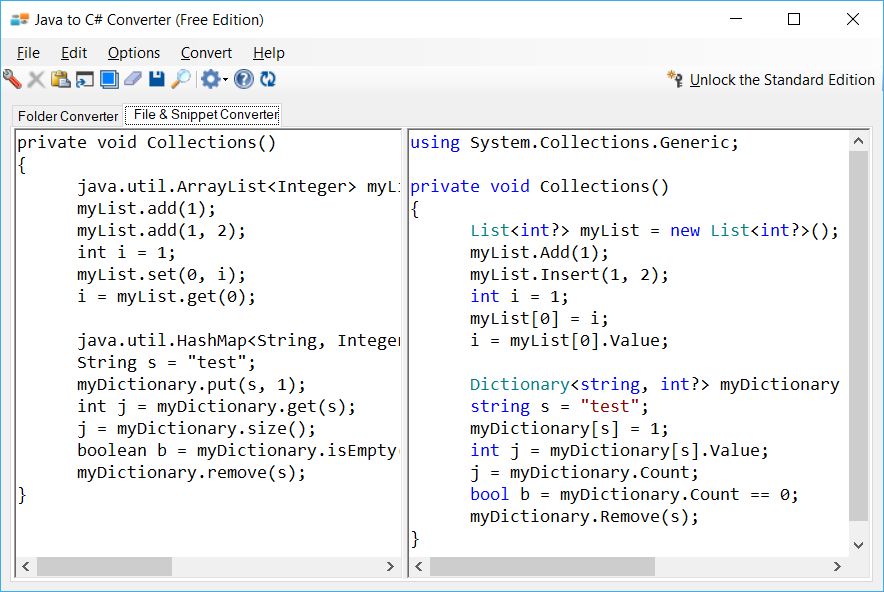
\includegraphics[scale=.4]{java-to-csharp-collections.png}
		\end{center}
		\caption{Chuyển đổi code Java sang C Scharp}
		\label{refhinh1}
	\end{figure}
\end{center}

\section{Công cụ dùng trong thực nghiệm}
%Phần này trình bày những công cụ được sử dụng để triển khai thực nghiệm như: công cụ sinh dữ liệu kiểm thử, môi trường lập trình, \dots
\subsection*{Microsoft Visual studio}
Microsoft Visual Studio là một môi trường phát triển tích hợp từ Microsoft. Nó được sử dụng để phát triển chương trình máy tính cho Microsoft Windows, cũng như các trang web, các ứng dụng web và các dịch vụ web. Visual Studio sử dụng nền tảng phát triển phần mềm của Microsoft như Windows API, Windows Forms, Windows Presentation Foundation, Windows Store và Microsoft Silverlight. Nó có thể sản xuất cả hai ngôn ngữ máy và mã số quản lý.

Visual Studio bao gồm một trình soạn thảo mã hỗ trợ IntelliSense cũng như cải tiến mã nguồn. Trình gỡ lỗi tích hợp hoạt động cả về trình gỡ lỗi mức độ mã nguồn và gỡ lỗi mức độ máy. Công cụ tích hợp khác bao gồm một mẫu thiết kế các hình thức xây dựng giao diện ứng dụng, thiết kế web, thiết kế lớp và thiết kế giản đồ cơ sở dữ liệu. Nó chấp nhận các plug-in nâng cao các chức năng ở hầu hết các cấp bao gồm thêm hỗ trợ cho các hệ thống quản lý phiên bản (như Subversion) và bổ sung thêm bộ công cụ mới như biên tập và thiết kế trực quan cho các miền ngôn ngữ cụ thể hoặc bộ công cụ dành cho các khía cạnh khác trong quy trình phát triển phần mềm.

\begin{center}
	\begin{figure}[htp]
		\begin{center}
			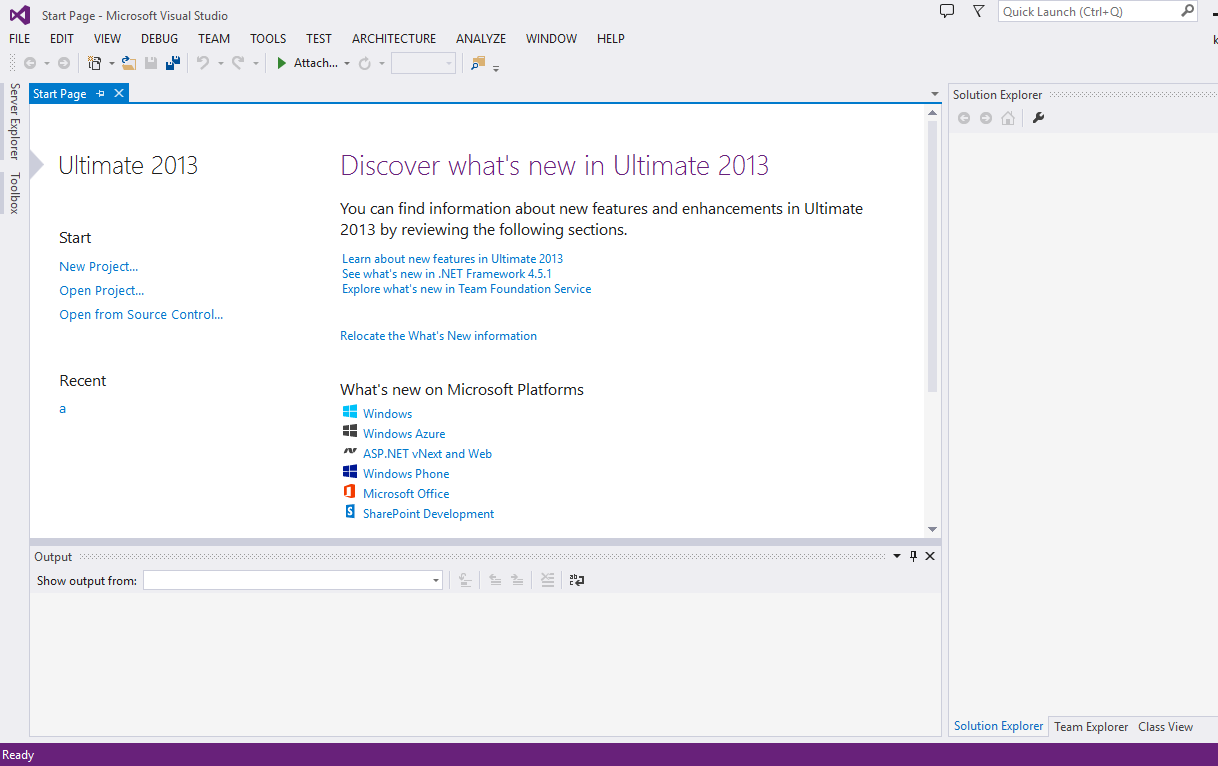
\includegraphics[scale=.3]{visualstudio.png}
		\end{center}
		\caption{Giao diện phần mềm Visual studio 2013}
		\label{refhinh1}
	\end{figure}
\end{center}

Visual Studio hỗ trợ nhiều ngôn ngữ lập trình khác nhau và cho phép trình biên tập mã và gỡ lỗi để hỗ trợ (mức độ khác nhau) hầu như mọi ngôn ngữ lập trình. Các ngôn ngữ tích hợp gồm có C,[1] C++ và C++/CLI (thông qua Visual C++), VB.NET (thông qua Visual Basic.NET), C thăng (thông qua Visual C thăng) và F thăng (như của Visual Studio 2010). Hỗ trợ cho các ngôn ngữ khác như J++/J thăng, Python và Ruby thông qua dịch vụ cài đặt riêng rẽ. Nó cũng hỗ trợ XML/XSLT, HTML/XHTML, JavaScript và CSS.

\subsection*{Ngôn ngữ lập trình C\# }
\subsubsection*{Tổng quan Ngôn ngữ C\# }
Quá trình dịch chương trình trong C\# là một ngôn ngữ lập trình hiện đại, được phát triển bởi Anders Hejlsberg cùng nhóm phát triển .Net Framework của Microsoft và được phê duyệt bởi European Computer Manufacturers Association (ECMA) và International Standards Organization (ISO).

Quá trình dịch chương trình trong C\#  được thiết kế cho các ngôn ngữ chung cơ sở hạ tầng (Common Language Infrastructure – CLI), trong đó bao gồm các mã (Executable Code) và môi trường thực thi (Runtime Environment) cho phép sử dụng các ngôn ngữ cấp cao khác nhau trên đa nền tảng máy tính và kiến trúc khác nhau.

\subsubsection*{Ngôn ngữ ra đời cùng với .NET}
\begin{itemize}
	\item Kết hợp C++ và Java.
	\item Hướng đối tượng.
	\item Hướng thành phần.
	\item Mạnh mẽ (robust) và bền vững (durable).
	\item Mọi thứ trong Quá trình dịch chương trình trong C\#  đều Object oriented.
	\item Chỉ cho phép đơn kế thừa.
	\item Lớp Object là cha của tất cả các lớp.
	\item Cho phép chia chương trình thành các thành phần nhỏ độc lập nhau.
	\item Mỗi lớp gói gọn trong một file, không cần file header như C/C++.
	\item Bổ sung khái niệm namespace để gom nhóm các lớp.
	\item Bổ sung khái niệm “property” cho các lớp.
	\item Khái niệm delegate và event.
\end{itemize}

\subsubsection*{Vai trò C\#  trong .NET Framework}
\begin{itemize}
	\item .NET runtime sẽ phổ biến và được cài trong máy client.
	\begin{enumerate}
		\item Việc cài đặt App C\#  như là tái phân phối các thành phần .NET
		\item Nhiều App thương mại sẽ được cài đặt bằng Quá trình dịch chương trình trong C\# .
	\end{enumerate}
	\item C\# tạo cơ hội cho tổ chức xây dựng các App Client/Server n-tier.
	\item Kết nối ADO.NET cho phép truy cập nhanh chóng và dễ dàng với SQL Server, Oracle…
	\item Cách tổ chức .NET cho phép hạn chế những vấn đề phiên bản.
	\item ASP.NET viết bằng Quá trình dịch chương trình trong C\#.
	\begin{enumerate}
		\item GUI thông minh.
		\item Chạy nhanh hơn (đặc tính của .NET)
		\item Mã ASP.NET không còn hỗn độn.
		\item Khả năng bẫy lỗi tốt, hỗ trợ mạnh trong quá trình xây dựng App Web.
	\end{enumerate}
\end{itemize}

\subsubsection*{Quá trình dịch chương trình trong C\# }
Mã nguồn C\# là các tập tin *.cs được trình biên dịch Compiler biên dịch thành các file *.dll hoặc *.exe, sau đó các file này được các hệ thống thông dịch CLR trên điều hành thông dịch qua mã máy và dùng kỹ thuật JIT (just-in-time) để tăng tốc độ.

\begin{center}
	\begin{figure}[htp]
		\begin{center}
			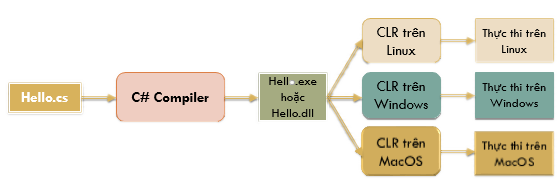
\includegraphics[scale=.4]{quatrinhthongdich.png}
		\end{center}
		\caption{Quá trình dịch chương trình trong C\#}
		
	\end{figure}
\end{center}

\subsubsection*{Các loại ứng dụng của C\#}
C\# có thể tạo ra được nhiều loại ứng dụng, trong đó có 3 kiểu phổ biến được nhiều nhà lập trình viên sử dụng nhất đó là: Console, Window và ứng dụng Web.
\begin{itemize}
	\item Ứng dụng Console là ứng dụng có giao diện text, chỉ xử lý nhập xuất trên màn hình Console, tương tự với các ứng dụng DOS trước đây. Loại ứng dụng Console thường đơn giản, ta có thể nhanh chóng tạo chương trình hiển thị kết xuất trên màn hình. Do đó, các minh hoạ, ví dụ ngắn gọn ta thường sử dụng dạng chương trình Console để thể hiện.
	\item Ứng dụng Windows Form là ứng dụng được hiển thị với giao diện cửa sổ đồ họa. Chúng ta chỉ cần kéo và thả các điều khiển (control) lên cửa sổ Form. Visual Studio sẽ sinh mã trong chương trình để tạo ra, hiển thị các thành phần trên cửa sổ.
	\item Ứng dụng Web, trên môi trường .NET cung cấp công nghệ ASP.NET, MVC giúp xây dựng những trang Web động. Để tạo ra một trang Web, người lập trình sử dụng ngôn ngữ biên dịch như C\# hoặc C\# để viết mã. Để đơn giản hóa quá trình xây dựng giao diện người dùng cho trang Web, .NET giới thiệu công nghệ Webform. Cách thức tạo ra các Web control tương tự như khi ta xây dựng ứng dụng trên Window Form.
\end{itemize}

\subsection{Công cụ sinh dữ liệu thử Pex}
\subsubsection*{Giới thiệu}
Khái niệm về DSE và các ứng dụng sử dụng kỹ thuật DSE đã có từ lâu, nhưng Pex là một ứng dụng mỡ rộng hơn so với các phiên bản DSE trước. Trong Visual Stuio, Pex đã được tích hợp như một Add-in, và có thể tạo ra các test case kết hợp với các bộ kiểm thử khác nhau như NUnit và MSTest. 

Cũng như với Unit Test, ta có thể viết các lớp kiểm thử chứa các ca kiểm thử tham số hóa. Với sự hỗ trợ của Pex ta có thể thực thi các ca kiểm thử tham số hóa đó. Tuy nhiên không giống việc thực thi các lớp kiểm thử chứa các Unit Test, Pex chỉ thực thi được một ca kiểm thử tham số hóa trong mỗi lần chạy.

\lstinputlisting[caption = {Ca kiểm thử tham số sử dụng Pex}]{TestPex.cs}

\subsubsection*{Các mẫu kiểm thử tham số hóa}
Viết các ca kiểm thử các tham số là một công việc tốn nhiều công sức. Để viết các ca kiểm thử các tham số hiệu quả, ta cần thực sự hiểu về mã cài đặt của chương trình mà ta muốn kiểm thử. Pex hỗ trợ cho chúng ta nhiều mẫu kiểm thử tham số khác nhau \cite{de2008parameterized}. Các mẫu được sử dụng nhiều nhất đó là mẫu AAA (Triple-A) và AAAA:
\begin{itemize}
	\item Với mẫu AAA (Arrange, Act, Assert) PUT được tổ chức thành 3 phần:
	\begin{itemize}
		\item Arrange: khởi tạo giá trị các biến sẽ sử dụng
		\item Act: dãy các lời gọi phương thức
		\item Assert: sự xác nhận
	\end{itemize}
	\item Với mẫu AAAA, một giả thuyết (Assume) được thêm vào để giới hạn miền giá trị của các tham số đầu vào.
\end{itemize}

\lstinputlisting[caption = {Mầu kiềm thử tham số hóa AAAA}]{AAAA.cs}

\subsubsection*{Lọn chọn đầu vào kiểm thử với Pex}
Đổ có thể sinh các đầu vào cụ thể cho các tham số Unit test, Pex cần phải phân tích chương trình với các tham số kiểm thử này. Có 2 kỹ thuật phân tích chương trình đó là:

\begin{itemize}
	\item Phân tích tĩnh (static analysis): Kiểm chứng một tính chất nào đó của chương trình bằng việc phân tích tất cả các đường đi thực thi. Kỹ thuật này coi các cảnh bảo (violations) là các lỗi (error).
	\item Phân tích động (dynamic analysis): Kiểm chứng một tính chất bằng việc phân tích một số đường đi thực thi. Đây là một kỹ thuật phân tích động hỗ trợ việc phát hiện ra các lỗi (bugs) nhưng không khẳng định được rằng có còn những lỗi khác hay không. Các kỹ thuật này thường không tìm ra được tất cả các lỗi.
\end{itemize}

Pex cài đặt một kỹ thuật phân tích chương trình bằng cách kết họp cả hai kỹ thuật phân tích chương trình ở trên gọi là thực thi tượng trưng động \cite{xie2009fitness}, \cite{godefroid2005dart}. Về bản chất Pex là một công cụ hỗ trợ kỹ thuật kiểm thử hộp hắng (white-box testing). Tương tự như kỹ thuật phân tích chương trình tĩnh, Pex chứng minh được rằng một tính chất được kiểm chứng trong tất cả các đường đi khả thi. Pex chỉ báo cáo (reporting) về các lỗi thực sự như với kỹ thuật phân tích chương trình động.

Pex sử dụng bộ xử lý ràng buộc Z3 \cite{de2008z3} kết họp với các lý thuyết toán học khác như hàm chưa định nghĩa, lý thuyết mảng, bit-vetor \cite{kroening2016decision} để giải quyết ràng buộc sinh ra trong quá trình thực thi tượng trưng động và sinh ra các đầu vào kiểm thử cụ thể cho tham số kiểm thử.

\subsubsection*{Mô hình ứng dụng Pex}

\begin{center}
	\begin{figure}[htp]
		\begin{center}
			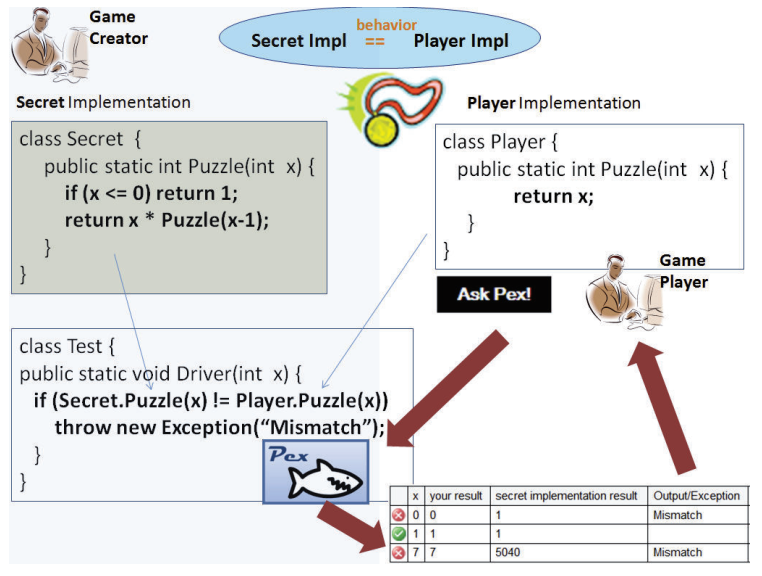
\includegraphics[scale=.4]{pex.png}
		\end{center}
		\caption{Mô hình ứng dụng Pex}
		
	\end{figure}
\end{center}

\section{Đánh giá kết quả thực nghiệm}
Phần này trình bày những kết quả đo được trên bộ dữ liệu thực nghiệm đã nêu trong Phần~\ref{sec:data}.

\section{Khả năng ứng dụng}
Phần này trình bày một số ứng dụng có thể của việc đo độ tương tự về hành vi của chương trình cùng hướng phát triển trong tương lai.

\subsection{Đánh giá tiến bộ trong lập trình}
Theo dõi sự tiến bộ trong học tập là một việc quan trọng, mà ngay cả với giảng viên và sinh viên công việc này là cả một quá trình. Có nhiều tiêu chí đánh giá sự tiến bộ trong học tập của sinh viên, trong đó tiêu chí về điểm số là một trong những tiêu chí cơ bản nhất. Một bảng thống kê điểm số, thành tích học tập của sinh viên sẽ thể hiện được sự tiến bộ của sinh viên trong học tập. Nhưng công việc chấm bài, tổng hợp, thống kê kết quả học tập của sinh viên mất rất nhiều thời gian của giảng viên. Một ứng dụng hỗ trợ chấm điểm, lưu trữ, thống kê và đánh giá điểm số của sinh viên là sẽ là một công cụ hỗ trợ đắc lực cho giảng viên trong công tác quản lý của mình. Nếu số liệu thống kê đánh giá kết quả các bài kiểm tra của sinh viên ngày càng cao, chứng tỏ sinh viên nắm được nội dung và kiến thức của chương trình đào tạo, và kết quả tốt sẽ là một động lực giúp cho sinh viên thêm tự tin, đam mê công việc học tập của mình. Ngược lại, nếu một sinh viên có điểm số ngày càng thấp chứng tỏ sinh viên đang có vấn đề trong kiến thức của của mình, lúc này tốt nhất sinh viên nên dừng lại không tiếp tục code và kiểm tra xem vấn đề mình đang gặp phải. 

\subsection{Xếp hạng tự động}
Công việc chấm điểm, phân loại và xếp hạng các bài kiểm tra của sinh viên cũng là một công việc tốn không ít công sức của giảng viên. Để giảm bớt gánh nặng cho giảng viên, chúng ta có thể sử dụng kết quả các độ đo trên từng bài tập của sinh viên như một phương pháp hỗ trợ công việc chấm điểm của từng sinh viên. Sự giống nhau về hành vi giữa chương trình của sinh viên và chương trình tham chiếu có thể là một yếu tố để phân loại sinh viên. Độ tương tự càng cao thì điểm số càng cao, các chỉ số này dựa hoàn toàn trên ngữ nghĩa của chương trình. Cách tiếp cận này giải quyết được các giới hạn trong trường hợp chương trình của sinh viên giống với chương trình tham chiếu, nhưng khác nhau về ngữ nghĩa. Các kết quả trong việc xếp hạng tự động sẽ giúp tiết kiệm được thời gian và giảng viên có thể đưa ra giải pháp giúp những sinh viên có điểm số thấp khắc phục được hạn chế đang gặp phải.

\subsection{Gợi ý giải pháp lập trình}
Thông thường, sinh viên thường viết code mới thực hiện chạy chương trình, lúc này sinh viên mới biết được kết quả đoạn code vừa thực hiện. Để hỗ trợ sinh viên viết code được tốt hơn, nếu như có một công cụ hỗ trợ kiểm tra theo thời gian thực và gửi thông báo lỗi nếu sinh viên viết code sai cú pháp hoặc chương trình bị lỗi không thể thực thi được. Ngoài ra, công cụ sẽ gợi ý giải pháp lập trình cho sinh viên bằng hình thức tự động tính toán thông báo kết quả các tham số đầu vào và đầu ra của chương trình so với chương trình được tham chiếu, đưa ra các số liệu về độ tương tự hành vi của chương trình.	

\subsection{Hướng phát triển}
Qua quá trình nghiên cứu và triển khai thực nghiệm, trong tương lai đề tài hướng tới phát triển thành một một ứng dụng hoàn chỉnh với việc bổ sung và hoàn thiện một số chức năng như sau:
\begin{itemize}
	\item Phát triển ứng dụng có thể chạy trên Web
	\item Chức năng quản lý sinh viên
	\item Quản lý kết quả học tập sinh viên
	\item Thêm chức năng đánh giá, xếp hạng tự động
	\item Thêm chức năng gợi ý giải pháp lập trình
	\item Cải tiến các độ đo để cho kết quả tốt hơn và nhanh hơn
	\item Phát triển thêm các nền tảng lập trình khác như java, c++..		
\end{itemize}

\section{Kết luận}
Qua quá trình nghiên cứu đề tài, có thể thấy rằng việc phát triển và ứng dụng các kỹ thuật đo đang dần trở nên phổ biến trong các chương trình giáo dục và đào tạo lập trình viên online. Những lợi ích, hiểu quả của việc đánh giá độ tương tự hành vi mang lại là rất thiết thực. Các kỹ thuật này không chỉ giúp quá trình giảng dạy của giảng viên được thuận lợi hơn, tiết kiệm được thời gian cũng như công sức trong công tác quản lý. Ngoài ra, sinh viên có được một môi trường tốt để tự rèn luyện, nâng cao các kỹ năng lập trình của bản thân. Việc tạo động lực giúp sinh viên có sự hứng thú và đam mê lập trình là rất cần thiết. Một khi sinh viên có tư duy và kỹ năng lập trình tốt, sinh viên sẽ tự tin vào năng lực của bản thân để tiếp tục phát phát triển sự nghiệp sau khi ra trường.

Đề tài đã thực hiện nghiên cứu rất nhiều vấn đề, nhưng trọng tâm đó là nghiên cứu sơ lượt về công cụ PEX của Microsoft, một công cụ sử dụng bộ xử lý ràng buộc Z3 \cite{de2008z3} kết họp với các lý thuyết toán học khác như hàm chưa định nghĩa, lý thuyết mảng, bit-vetor \cite{kroening2016decision} để giải quyết các ràng buộc sinh ra trong quá trình thực thi tượng trưng động, và sinh ra các đầu vào kiểm thử có độ phủ cao cho tham số kiểm thử của chương trình. Ứng dụng công cụ PEX nghiên cứu các kỹ thuật đo độ tương tự hành vi của chương trình, sao cho kết quả các độ đo được chính xác hơn. Từ khả năng xử lý của các độ đo, xây dựng một công cụ để minh họa cho các kỹ thuật đo.

Những nội dung trình bày trong luận văn này không tránh khỏi còn nhiều thiếu xót vì lý do nhiều lý do khách quan khác nhau như: Thời gian thực hiện đề tài hạn hẹp; lượng kiến thức cơ sở để triển khai thực hiện rất lớn; cùng với đó là kinh nghiệm của bản thân trong việc thực hiện các đề tài chưa có. Tuy nhiên, với sự hướng dẫn tận tình của giáo viên hướng dẫn, đề tài đã đạt được nhiều nội dung quan trọng, và có thể mở ra nhiều hướng nghiên cứu và phát triển khác của đề tài. Như việc mở rộng DSE để hỗ trợ việc thực thi tượng trưng các chương trình có dữ liệu phức tạp, hay có số vòng lặp lớn. Cải tiến kỹ thuật đo, kết hợp với kỹ thuật DSE để có kết quả độ đo được chính xác hơn, nhạy hơn. Tiếp tục nghiên cứu, phát triển để thực các kỹ thuật đo trên các ngôn ngữ khác như Java, C++ và chạy được trên nền tảng PC, Web. 



\bibliographystyle{plain}
\bibliography{biblio}
\todo{Trích dẫn bài báo}
\nocite{*} % dùng tạm thời


\appendix

\chapter{Quyết định XXX}
\newpage
\chapter*{QUYẾT ĐỊNH GIAO LUẬN VĂN} 
\addcontentsline{toc}{chapter}{QUYẾT ĐỊNH GIAO LUẬN VĂN}
\todo{scan quyet dinh sang pdf và include}
%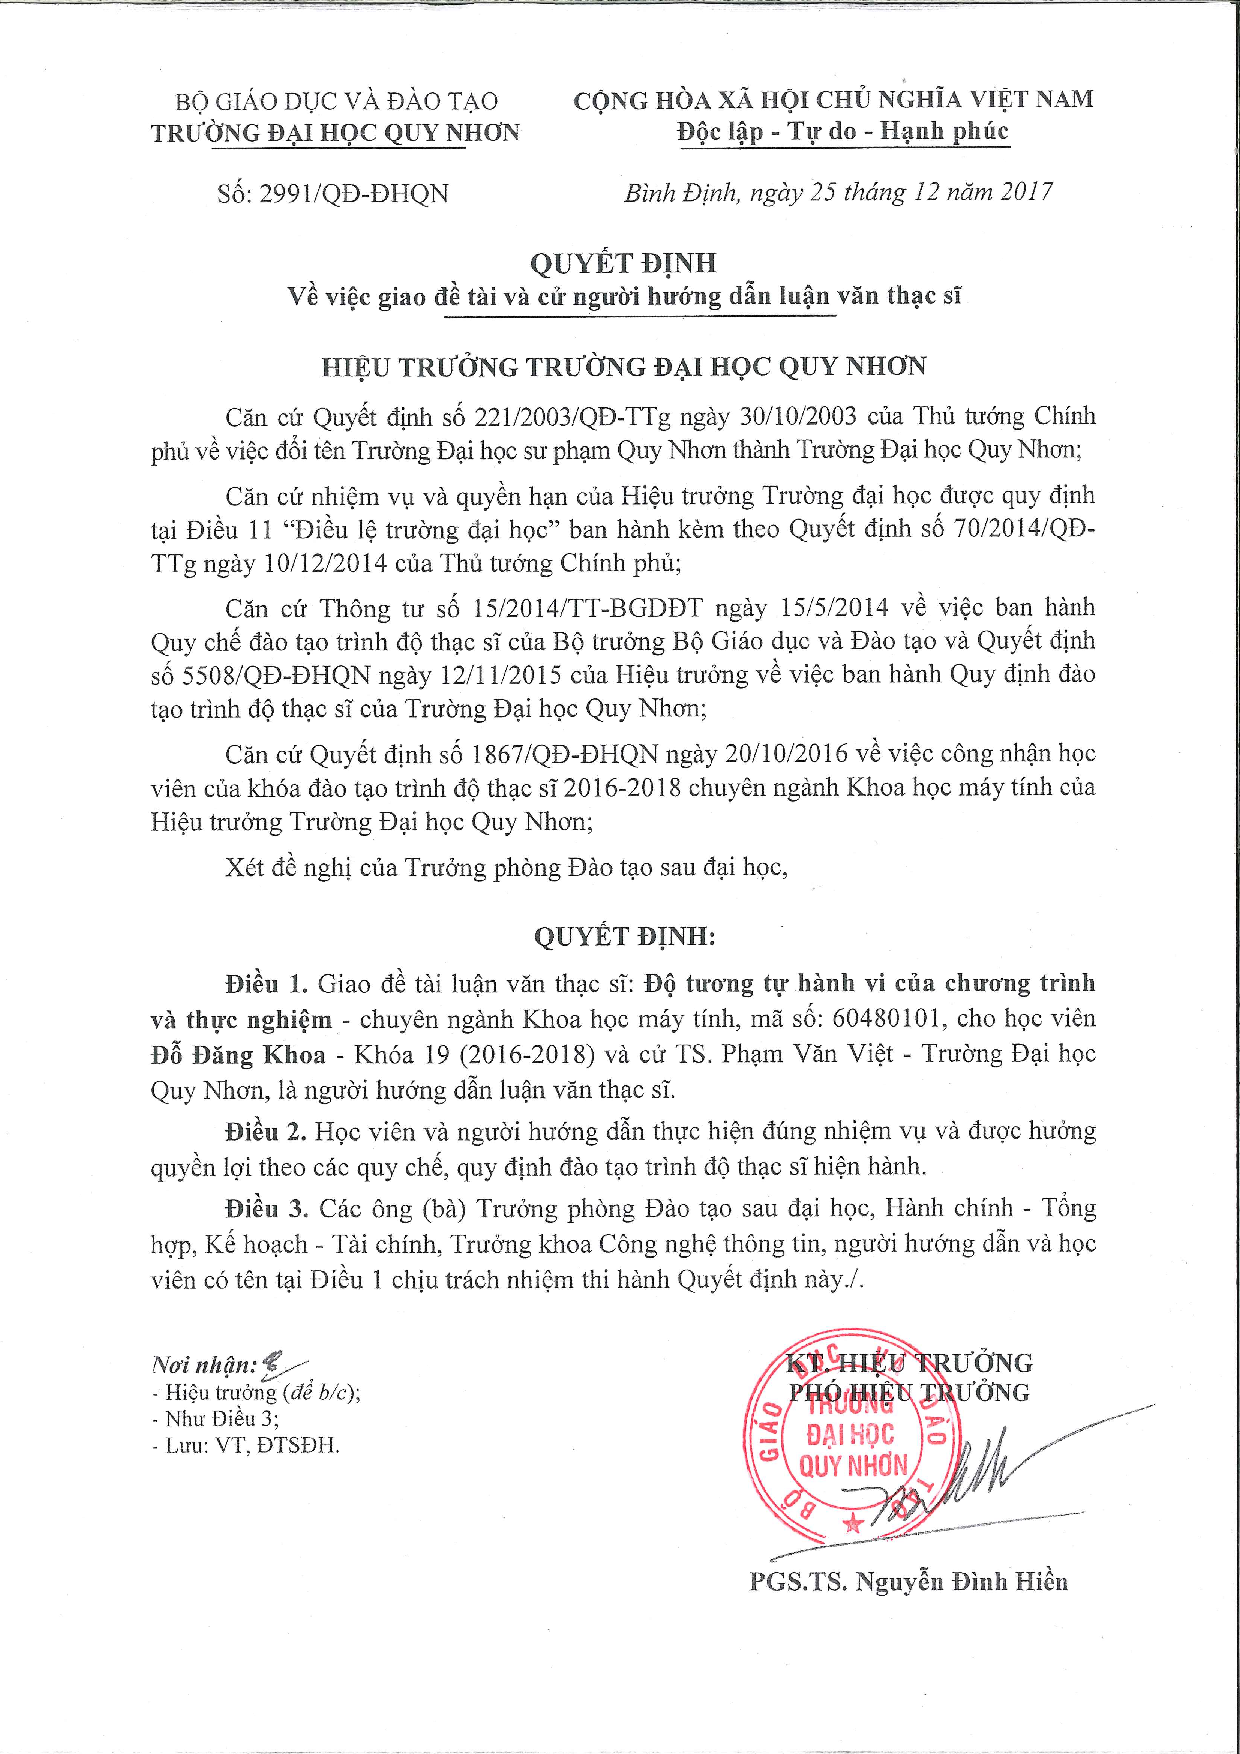
\includepdf{quyetdinh.pdf}

\chapter{Phụ lục XXX}
\begin{center}
	\textbf{PHỤ LỤC}
\end{center}

\chapter{Một số mã lệnh quan trọng}
\lstinputlisting[caption = {Mã lệnh tạo project của sinh viên}]{MakeProjects.cs}

\lstinputlisting[caption= {Mã lệnh tạo project chương trình tham chiếu}]{MakeSecretProjects.cs}

\lstinputlisting[caption={Mã lệnh build project của sinh viên}]{BuildProjects.cs}

\lstinputlisting[caption={Mã lệnh build project chương trình tham chiếu}]{BuildSecretProjects.cs}

\lstinputlisting[caption={Mã lệnh build project chương trình hợp thành}]{BuildMetaProjects.cs}

\lstinputlisting[caption={Mã lệnh thực thi DSE trên chương trình hợp thành}]{RunPexOnMetaProjects.cs}

\lstinputlisting[caption={Mã lệnh phép đo RS}]{ComputeMetric3.cs}

\lstinputlisting[caption={Mã lệnh phép đo SSE}]{ComputeMetric2.cs}

\lstinputlisting[caption={Mã lệnh phép đo PSE}]{ComputeMetric1.cs}

 


\end{document}

